\documentclass[a4paper,12pt]{article}

%% Language and font encodings
\usepackage[english, russian]{babel}
\usepackage[utf8x]{inputenc}
\usepackage{blindtext}
\usepackage[T1]{fontenc}
\usepackage[T2A]{fontenc}
\usepackage[a4paper,top=1.5 cm,bottom=2cm,left=3cm,right=3cm,marginparwidth=1.75cm]{geometry}
%% Useful packages
\usepackage{amsmath, amssymb}
\usepackage{wrapfig}
\usepackage{graphicx}
\usepackage[usenames]{color}
\usepackage[T1]{fontenc}
\usepackage{tikz}
\usetikzlibrary{arrows}
\usetikzlibrary{decorations.pathreplacing}
\usepackage[T2A]{fontenc}
\usepackage{color}
\usepackage{circuitikz} 
\usetikzlibrary{circuits}
\usetikzlibrary{circuits.ee}
\usetikzlibrary{circuits.ee.IEC}
\usetikzlibrary{circuits.logic.IEC}
\graphicspath{{pic/}}
\definecolor{water} {rgb} {0.667, 0.855, 1}
\usepackage{pgfplots}
\usepackage{pgfplotstable}

\title{ИНТЕРФЕРОМЕТР МАЙКЕЛЬСОНА}
\date{Работа 4.3.1}
\author{Ляликова Ирина, Б05-911}
\begin{document}
	
	\vspace{0.5 cm}
	\maketitle
	\vspace{0.5 cm}
	
	\textbf{Цель работы:} изучение двухлучевой интерференции, определение длины волны, проверка эффекта Доплера.
	
	\textbf{В работе используются:} интерферометр Майкельсона с подвижным зеркалом, лазер ЛГН-203, фотоумножитель ФЭУ-68 с блоком питания, частотомер Ч3-54, линзы.
	
	\section*{Теоретическое введение и установка}
	
	Схема устройства интерферометра приведена на рис. 1. Источником света служит лазер ЛГ. Лазер излучает узкий пучок света, который фокусируется линзой Л$_1$. В фокусе этой линзы возникает точечный источник света 5. Сферическая световая волна от источника 5 падает на делительную призму П и делится её диагональной гранью на две волны --- отражённую 1 и проходящую 2. Волна 1 отражается от зеркала З$_1$, возвращается к призме П, частично проходит сквозь неё и попадает на экран Э. Волна 2 отражается от зеркала 3$_2$, частично отражается от призмы П и также попадает на экран. Световые волны 1 и 2 испускаются одним источником 5, и они когерентны между собой. Эти волны создают на экране Э интерференционную картину. Для увеличения масштаба интерференционной картины может быть использована линза Л$_2$.
	
		\begin{figure}[h]
		\begin{center}
			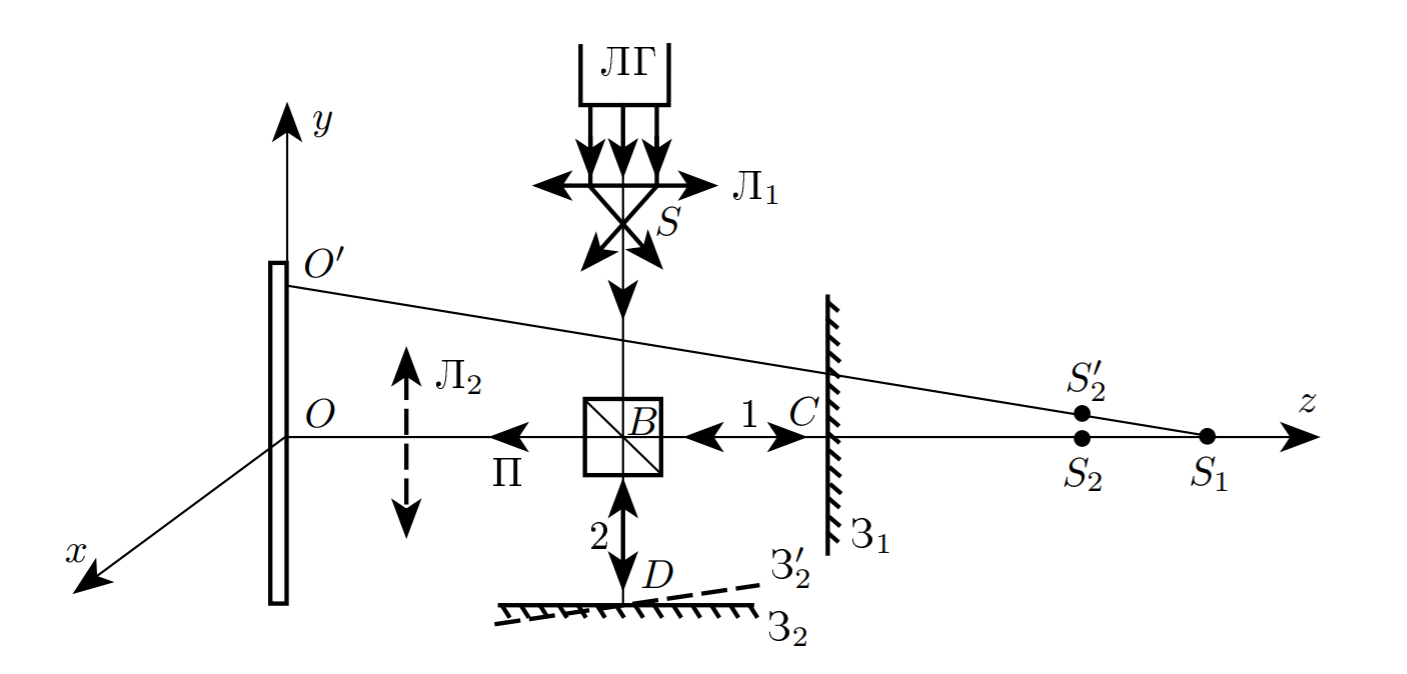
\includegraphics[width = 0.7\textwidth]{424-1.png}
			\caption{Схема интерферометра}
		\end{center}
	\end{figure}
	
	Зеркало З$_1$ установлено перпендикулярно падающему лучу. Оно может перемещаться вдоль луча. Это зеркало в дальнейшем будет называться подвижным. Зеркало 3$_2$ вдоль направления падающего луча не перемещается. Его, однако, можно наклонять по отношению к лучу.
	
	\subsection*{Экспериментальная установка}
	Схема экспериментальной установки приведена на рис. 2. Источником света служит гелий-неоновый лазер ЛГН-203. Его излучение обладает большой длиной когерентности, что позволяет получать хорошо различимую глазом интерференционную картину при разности хода в десятки сантиметров. Неподвижное зеркало 3$_2$, поворачивается микрометрическими винтами М, (относительно горизонтальной) и М, (относительно вертикальной оси). Зеркало З$_1$ установлено перпендикулярно падающему лучу.
	\begin{figure}[h]
		\begin{center}
			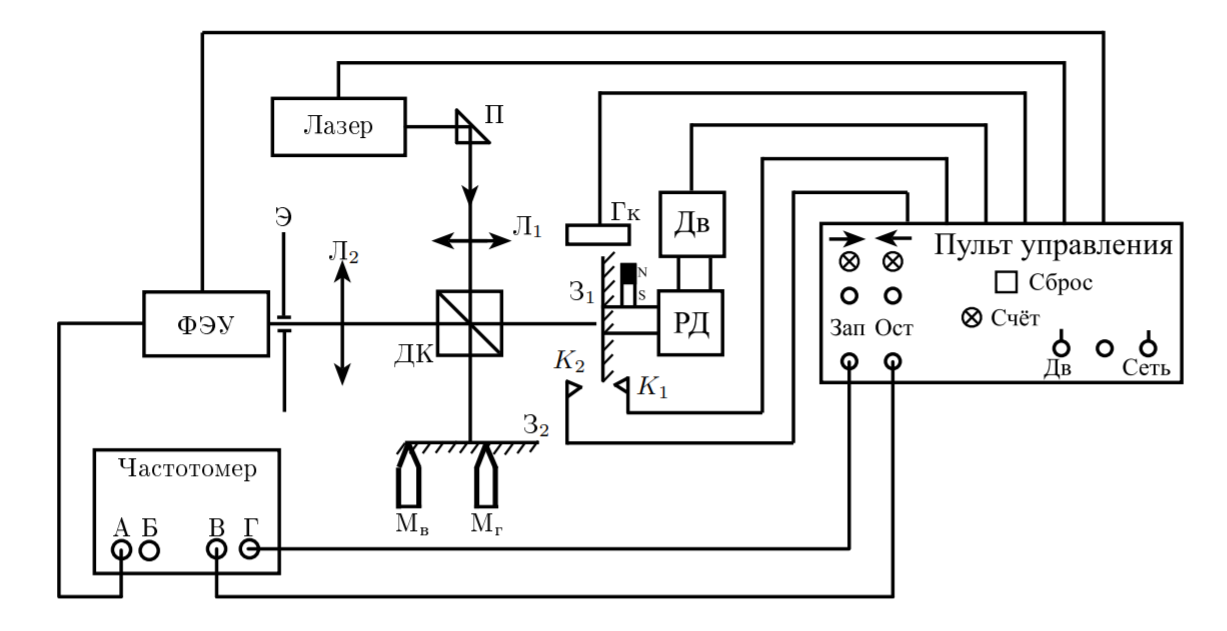
\includegraphics[width = 0.85\textwidth]{424-2.png}
			\caption{Схема установки}
		\end{center}
	\end{figure}
	 Оно может передвигаться вдоль луча с помощью микрометрического винта, соединённого с двигателем Дв через муфту и редуктор РД, позволяющий менять скорость движения зеркала. Двигатель питается от сети через блок питания пульта управления. Концевые контакты К$_1$ и К$_2$ меняют направление движения зеркала на обратное. Включение лазера и двигателя производится с пульта управления. Сигнальные лампочки указывают, в какую сторону движется зеркало.
	 
	 Интерференционная картина наблюдается на экране Э. Она может быть увеличена с помощью линзы Л$_2$. В этом случае на экране в увеличенном масштабе воспроизводится интерференционная картина, которая создаётся перед линзой в плоскости, сопряжённой экрану. Линза закреплена на съёмном столике, её фокусное расстояние 4,3 см.
	 
	 Для регистрации изменения интенсивности света используется фотоэлектронный умножитель ФЭУ-68, установленный непосредственно за экраном. Свет на окно ФЭУ попадает через небольшое отверстие в центре экрана. Для питания ФЭУ используется высоковольтный выпрямитель. Выпрямитель включается тумблером «Сеть» на пульте управления.
	 
	 Периодическое изменение интенсивности света, возникающее при движении зеркала З1, приводит к такому же изменению сигнала ФЭУ. Число периодов изменения интенсивности света пересчитывается частотомером Ч3-54. Частотомер может работать в одном из трёх режимов.
	 \begin{enumerate}
	 	\item Он может измерять число импульсов, поступающих на его входы (А или Б) за некоторый промежуток времени (его продолжительность определяется поступлением сигналов на управляющие входы В и Г).
	 	\item С помощью частотомера можно измерять промежутки времени. Для таких измерений в прибор встроен кварцевый генератор. Частотомер измеряет время, прошедшее между поступлением сигналов на его управляющие входы, подсчитывая соответствующее число импульсов кварцевого генератора.
	 	\item Наконец, частотомер может измерять частоту сигнала, поступающего на его вход, сравнивая число периодов исследуемого сигнала с числом импульсов кварцевого генератора. 
	 	
 	\end{enumerate}
	 	
	 	Для получения управляющих сигналов используется геркон Гк (герметичный магнитоуправляемый контакт). Схема работает следующим образом. На отсчётной головке микрометрического винта зеркала З$_1$ закреплён небольшой магнит. Головка вращается вместе с винтом. После срабатывания концевого контакта. К$_2$ зеркало начинает двигаться от экрана. При приближении магнита к геркону вырабатывается управляющий сигнал, который подаётся через схему пульта управления на вход В частотомера. Частотомер начинает счёт импульсов. После того, как с помощью геркона зарегистрировано 32 оборота ходового винта, на вход Г частотомера подаётся сигнал на окончание счёта. После срабатывания концевого контакта К, зеркало начинает движение к экрану. На этом участке движения счёт импульсов не производится. Один оборот микрометрического винта приводит к перемещению зеркала на 1 мм. Таким образом, полное перемещение зеркала З$_1$ составляет $l = 32$ мм.
	 	
	 	
	 	\section*{Ход работы}
	 	\subsection*{Юстировка системы}
	 	\begin{enumerate}
	 		\item Включили блок питания установки (тумблер слева от частотомера).
	 		\item Убедились, что луч от поворотной призмы (П на рис.2) идёт параллельно столу на высоте $100\pm2$ мм (при этом линза Л$_1$ и делительный кубик сняты).
	 		\item Установили оправу с зеркалом~З$_2$ перпендикулярно лучу поворотом оправы в зеркале.
	 		\item Установили делительный кубик в центре системы и определили его положение относительно вертикали: луч от поворотной призмы, отразившись от полупрозрачной грани кубика, попадает на центр подвижного зеркала~З$_1$, а прямой луч, отразившись от зеркала~З$_2$, --- на центр экрана.
	 	\end{enumerate}
 	\subsection*{Исследование интерференционной картины}
 	\begin{enumerate}
 		\item Чтобы увеличить интерференционную картину, установили между экраном и кубиком столик с линзой Л$_2$.
 		\item Слегка проворачивая вручную муфту двигателя, установили в центре экрана оказалось тёмное пятно. Приложили к экрану лист бумаги, на котором проведён крест из взаимно перпендикулярных линий. Совместили центр креста с центром колец, наметили положение пяти-шести первых тёмных колец и измерили их радиусы. $\Delta r_n = 0{,}5$ мм.
 		\begin{center}
 			\begin{tabular}{|c|c|c|c|c|c|l|}
 				\hline
 				$n$ & 1 & 2 & 3 & 4 & 5 & 6 \\ \hline
 				$r_n$, мм & 1,5 & 4,0 & 5,5 & 6,5 & 7,5 & 8,5 \\ \hline
 			\end{tabular}
 		\end{center}
 		
 		Построим график квадрата радиуса кольца от его номера чтобы проверить справедливость формулы 
 		\begin{equation*}
 		r_n\approx \sqrt{\dfrac{2nL(L-a)}{m_0}},
 		\end{equation*}
 		где $m_0=a/\lambda$ --- порядок интерференции. 
 		\begin{figure}[h]
 			\begin{center}
 				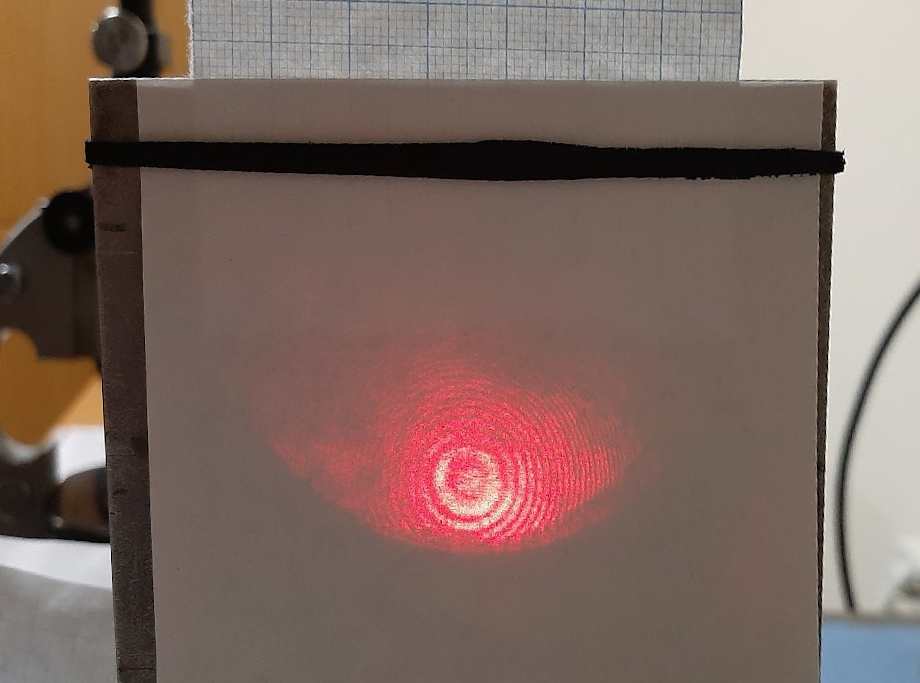
\includegraphics[width = 0.5\textwidth]{4.jpg}
 				\caption{Интерференционная картина}
 			\end{center}
 		\end{figure}
 		
 		\begin{figure}[!htb] \centering
 			\begin{tikzpicture}
 			\begin{axis}[
 			width=15cm,
 			height=8cm,
 			xlabel={$n$},
 			ylabel={$r^2$, мм$^2$},
 			grid=major
 			]
 			\addplot +[
 			blue!20!black,
 			mark = *,
 			only marks,
 			] plot [
 			error bars/.cd,
 			y dir=both,
 			y explicit,
 			] table [
 			x = n,
 			y = l2,
 			y error = dl,
 			] {424.dat};
 			\addplot +[
 			blue!20!black,
 			mark = 0,
 			] table [
 			y={create col/linear regression={y=l2}}]
 			{424.dat};
 			\end{axis}
 			\end{tikzpicture}
 			\caption{Зависимость квадрата радиуса от номера кольца}
 		\end{figure}
 	\end{enumerate}
 По линейности графика можно судить о том, что формула верна.
 \subsection*{Измерение длины волны лазерного излучения}
 \begin{enumerate}
 	\item Получили картину колец без столика с линзой Л$_2$. Установили частотомер в режим счёта импульсов. Включили двигатель тумблерами «Сеть» и «Дв» на пульте управления. Проследили за работой схемы управления двигателем при 2-3 изменениях направления движения зеркала.
 	\item Определили по табло частотомера число колец $N$, прошедших через центр экрана, (через вход «ФЭУ») за время движения зеркала. В выбранном режиме работы частотомер включается при отходе зеркала от контакта К$_2$ и выключается после 32-го оборота ходового винта. Перемещение зеркала $l = 32$ мм. Запуск частотомера происходит автоматически: после вспышки индикатора «$\rightarrow$» (движение от экрана) зажигается лампочка селектора частотомера и начинается отсчёт.
 	
 	Провели измерения числа интерференционных полос $N$, проходящих через центр экрана. Отключили двигатель. Результаты измерений представлены в таблице ниже:
 	\begin{center}
 		\begin{tabular}{|c|c|c|c|c|c|l|l|l|}
 			\hline
 			$n$ & 1 & 2 & 3 & 4 & 5 & 6 & 7 & 8 \\ \hline
 			$N\cdot 10^3$ & 144 & 147 & 150 & 147 & 144 & 137 & 146 & 147 \\ \hline
 		\end{tabular}
 	\end{center}
 	
 	По результатам этих измерений $<N>=145\pm4$ нашли длину волны лазерного излучения, используя формулу 
 	\begin{equation}
 	l=vT=N\lambda/2.
 	\end{equation}
 	Сравнили полученный результат для длины волны $\lambda=440\pm12$ нм с паспортным: $\lambda = 632{,}8$~нм.
 	
 \end{enumerate}
\subsection*{Исследование эффекта Доплера}
Измерения сводятся к определению частоты колебаний интенсивности света на входе ФЭУ при движении зеркала и определению скорости этого движения. Для проверки результатов измерений используется формула (1). При измерении частоты частотомер работает в режиме измерения частоты, при измерении скорости — в режиме измерения времени (скорость рассчитывается по времени, которое требуется для перемещения зеркала на расстояние $l = 32$ мм).

\begin{enumerate}
	\item Установили максимальную скорость передвижения зеркала (рычаг регулятора скорости --- в положение 1). Включили двигатель.
	\item При выбранном значении скорости сначала измерили время передвижения зеркала на расстояние $l$, затем доплеровскую частоту --- частоту изменения яркости света, падающего на ФЭУ (число полос, проходящих через ФЭУ за 1 с). Повторили измерения.
	Время передвижения $t=42{,}3\pm0{,}2$ c., откуда получаем скорость зеркала $v_1=0{,}757\pm0{,}004$ мм/с. Результаты измерения частоты:
	\begin{center}
		\begin{tabular}{|c|c|c|c|c|c|c|c|c|}
			\hline
			$n$ & 1 & 2 & 3 & 4 & 5 & 6 & 7 & 8 \\ \hline
			$\nu_1$, кГц & 2,462 & 2,480 & 2,473 & 2,509 & 2,510 & 2,533 & 2,526 & 2,594 \\ \hline
			$\nu_2$, кГц & 3,013 & 2,925 & 2,999 & 3,032 & 2,964 & 2,988 & 2,930 & 3,015 \\ \hline
		\end{tabular}
	\end{center}
	Тогда получаем, что для такой скорости 
	\begin{equation*}
	<\nu_1> = 2{,}511\pm0{,}002\text{ кГц},\;\;\;\;\;\; <\nu_2>=2{,}983\pm0{,}002\text{ кГц}.
	\end{equation*} 
	Тогда рассчитываем среднюю частоту $<\nu> = 2{,}724\pm0{,}002$ кГц, а так же доплеровскую разность частот $\Delta\nu=0{,}4270\pm0{,}0004$ кГц.
	\item Повторили измерения для 2-й скорости передвижения зеркала.
	\begin{equation*}
	t = 81{,}8\pm0{,}2 \text{ с.}, \;\;\;\;\;\; v = 0{,}391\pm0{,}001\text{ мм/с}.
	\end{equation*}
	\begin{center}
		\begin{tabular}{|c|c|c|c|c|c|c|c|c|}
			\hline
			$n$ & 1 & 2 & 3 & 4 & 5 & 6 & 7 & 8 \\ \hline
			$\nu_1$, кГц & 1,709 & 1,730 & 1,775 & 1,723 & 1,653 & 1,599 & 1,652 & 1,725 \\ \hline
			$\nu_2$, кГц & 1,555 & 1,664 & 1,658 & 1,677 & 1,507 & 1,576 & 1,668 & 1,664 \\ \hline
		\end{tabular}
	\end{center}
	\begin{equation*}
	<\nu_1> = 1{,}621\pm0{,}004\text{ кГц},\;\;\;\;\;\; <\nu_2>=1{,}696\pm0{,}003\text{ кГц}.
	\end{equation*} 
	\begin{equation*}
	<\nu> = 1{,}659\pm0{,}004\text{ кГц},\;\;\;\;\;\; \Delta\nu=0{,}0375\pm0{,}0001\text{ кГц}.
	\end{equation*}
	
	
	\item Повторили измерения для 3-й скорости передвижения зеркала.
		\begin{equation*}
	t = 224{,}8\pm0{,}2 \text{ с.}, \;\;\;\;\;\; v = 0{,}1423\pm0{,}0002\text{ мм/с}.
	\end{equation*}
	\begin{center}
		\begin{tabular}{|c|c|c|c|c|c|c|c|c|}
			\hline
			$n$ & 1 & 2 & 3 & 4 & 5 & 6 & 7 & 8 \\ \hline
			$\nu_1$, кГц & 1,577 & 1,802 & 1,643 & 1,774 & 1,708 & 1,603 & 1,666 & 1,645 \\ \hline
			$\nu_2$, кГц & 1,465 & 1,318 & 1,554 & 1,204 & 1,183 & 1,497 & 1,537 & 1,462 \\ \hline
		\end{tabular}
	\end{center}
	\begin{equation*}
	<\nu_1> = 1{,}677\pm0{,}005\text{ кГц},\;\;\;\;\;\; <\nu_2>=1{,}40\pm0{,}02\text{ кГц}.
	\end{equation*} 
	\begin{equation*}
	<\nu> = 1{,}54\pm0{,}01\text{ кГц},\;\;\;\;\;\; \Delta\nu=0{,}277\pm0{,}002\text{ кГц}.
	\end{equation*}
	\item Тут предлагалось построить график доплеровской разности частот в зависимости от скорости, но это выглядит совсем нецелесообразно, потому что среди трёх точек средняя частота одной сильно отличается от остальных по необъяснимым причинам, так что информативность такого графика будет невысокой.
\end{enumerate}
\section*{Вывод}
Провели опыт по двухлучевой интеренции Майкельсона, получили интреференционную картину, провели измерения радиусов колец для проверки формулы. Полученная зависимость подтверждает теоретическую. 

С помощью частотометра провели измерение числа колец, проходящих за единицу времени через точку на экране при разных скоростях движения зеркала. Рассчитали длину волны лазера, исходя из полученных результатов, получили заметное расхождение с паспортными данными. Это может быть связано с неточностью измерения частоты вследствие нечёткой интерверенционной картины. 

Провели измерения для различных направлений движения, качетсвенно убедились в существовании эффекта Доплера. Количественные измерения не дали удовлетворительных результатов.  
\end{document}
